\documentclass[1p]{elsarticle_modified}
%\bibliographystyle{elsarticle-num}

%\usepackage[colorlinks]{hyperref}
%\usepackage{abbrmath_seonhwa} %\Abb, \Ascr, \Acal ,\Abf, \Afrak
\usepackage{amsfonts}
\usepackage{amssymb}
\usepackage{amsmath}
\usepackage{amsthm}
\usepackage{scalefnt}
\usepackage{amsbsy}
\usepackage{kotex}
\usepackage{caption}
\usepackage{subfig}
\usepackage{color}
\usepackage{graphicx}
\usepackage{xcolor} %% white, black, red, green, blue, cyan, magenta, yellow
\usepackage{float}
\usepackage{setspace}
\usepackage{hyperref}

\usepackage{tikz}
\usetikzlibrary{arrows}

\usepackage{multirow}
\usepackage{array} % fixed length table
\usepackage{hhline}

%%%%%%%%%%%%%%%%%%%%%
\makeatletter
\renewcommand*\env@matrix[1][\arraystretch]{%
	\edef\arraystretch{#1}%
	\hskip -\arraycolsep
	\let\@ifnextchar\new@ifnextchar
	\array{*\c@MaxMatrixCols c}}
\makeatother %https://tex.stackexchange.com/questions/14071/how-can-i-increase-the-line-spacing-in-a-matrix
%%%%%%%%%%%%%%%

\usepackage[normalem]{ulem}

\newcommand{\msout}[1]{\ifmmode\text{\sout{\ensuremath{#1}}}\else\sout{#1}\fi}
%SOURCE: \msout is \stkout macro in https://tex.stackexchange.com/questions/20609/strikeout-in-math-mode

\newcommand{\cancel}[1]{
	\ifmmode
	{\color{red}\msout{#1}}
	\else
	{\color{red}\sout{#1}}
	\fi
}

\newcommand{\add}[1]{
	{\color{blue}\uwave{#1}}
}

\newcommand{\replace}[2]{
	\ifmmode
	{\color{red}\msout{#1}}{\color{blue}\uwave{#2}}
	\else
	{\color{red}\sout{#1}}{\color{blue}\uwave{#2}}
	\fi
}

\newcommand{\Sol}{\mathcal{S}} %segment
\newcommand{\D}{D} %diagram
\newcommand{\A}{\mathcal{A}} %arc


%%%%%%%%%%%%%%%%%%%%%%%%%%%%%5 test

\def\sl{\operatorname{\textup{SL}}(2,\Cbb)}
\def\psl{\operatorname{\textup{PSL}}(2,\Cbb)}
\def\quan{\mkern 1mu \triangleright \mkern 1mu}

\theoremstyle{definition}
\newtheorem{thm}{Theorem}[section]
\newtheorem{prop}[thm]{Proposition}
\newtheorem{lem}[thm]{Lemma}
\newtheorem{ques}[thm]{Question}
\newtheorem{cor}[thm]{Corollary}
\newtheorem{defn}[thm]{Definition}
\newtheorem{exam}[thm]{Example}
\newtheorem{rmk}[thm]{Remark}
\newtheorem{alg}[thm]{Algorithm}

\newcommand{\I}{\sqrt{-1}}
\begin{document}

%\begin{frontmatter}
%
%\title{Boundary parabolic representations of knots up to 8 crossings}
%
%%% Group authors per affiliation:
%\author{Yunhi Cho} 
%\address{Department of Mathematics, University of Seoul, Seoul, Korea}
%\ead{yhcho@uos.ac.kr}
%
%
%\author{Seonhwa Kim} %\fnref{s_kim}}
%\address{Center for Geometry and Physics, Institute for Basic Science, Pohang, 37673, Korea}
%\ead{ryeona17@ibs.re.kr}
%
%\author{Hyuk Kim}
%\address{Department of Mathematical Sciences, Seoul National University, Seoul 08826, Korea}
%\ead{hyukkim@snu.ac.kr}
%
%\author{Seokbeom Yoon}
%\address{Department of Mathematical Sciences, Seoul National University, Seoul, 08826,  Korea}
%\ead{sbyoon15@snu.ac.kr}
%
%\begin{abstract}
%We find all boundary parabolic representation of knots up to 8 crossings.
%
%\end{abstract}
%\begin{keyword}
%    \MSC[2010] 57M25 
%\end{keyword}
%
%\end{frontmatter}

%\linenumbers
%\tableofcontents
%
\newcommand\colored[1]{\textcolor{white}{\rule[-0.35ex]{0.8em}{1.4ex}}\kern-0.8em\color{red} #1}%
%\newcommand\colored[1]{\textcolor{white}{ #1}\kern-2.17ex	\textcolor{white}{ #1}\kern-1.81ex	\textcolor{white}{ #1}\kern-2.15ex\color{red}#1	}

{\Large $\underline{12a_{0805}~(K12a_{0805})}$}

\setlength{\tabcolsep}{10pt}
\renewcommand{\arraystretch}{1.6}
\vspace{1cm}\begin{tabular}{m{100pt}>{\centering\arraybackslash}m{274pt}}
\multirow{5}{120pt}{
	\centering
	\includegraphics[width=112pt]{../../../GIT/diagram.site/Diagrams/png/1606_12a_0805.png}\\
\ \ \ A knot diagram\footnotemark}&
\allowdisplaybreaks
\textbf{Linearized knot diagam} \\
\cline{2-2}
 &
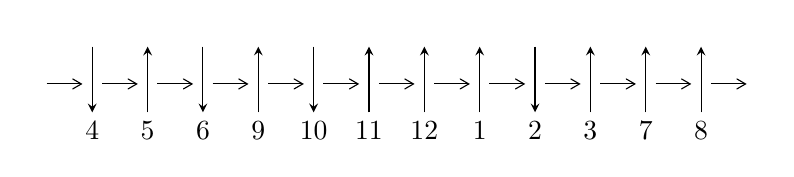
\begin{tikzpicture}[x=20pt, y=17pt]
	% nodes
	\node (C0) at (0, 0) {};
	\node (C1) at (1, 0) {};
	\node (C1U) at (1, +1) {};
	\node (C1D) at (1, -1) {4};

	\node (C2) at (2, 0) {};
	\node (C2U) at (2, +1) {};
	\node (C2D) at (2, -1) {5};

	\node (C3) at (3, 0) {};
	\node (C3U) at (3, +1) {};
	\node (C3D) at (3, -1) {6};

	\node (C4) at (4, 0) {};
	\node (C4U) at (4, +1) {};
	\node (C4D) at (4, -1) {9};

	\node (C5) at (5, 0) {};
	\node (C5U) at (5, +1) {};
	\node (C5D) at (5, -1) {10};

	\node (C6) at (6, 0) {};
	\node (C6U) at (6, +1) {};
	\node (C6D) at (6, -1) {11};

	\node (C7) at (7, 0) {};
	\node (C7U) at (7, +1) {};
	\node (C7D) at (7, -1) {12};

	\node (C8) at (8, 0) {};
	\node (C8U) at (8, +1) {};
	\node (C8D) at (8, -1) {1};

	\node (C9) at (9, 0) {};
	\node (C9U) at (9, +1) {};
	\node (C9D) at (9, -1) {2};

	\node (C10) at (10, 0) {};
	\node (C10U) at (10, +1) {};
	\node (C10D) at (10, -1) {3};

	\node (C11) at (11, 0) {};
	\node (C11U) at (11, +1) {};
	\node (C11D) at (11, -1) {7};

	\node (C12) at (12, 0) {};
	\node (C12U) at (12, +1) {};
	\node (C12D) at (12, -1) {8};
	\node (C13) at (13, 0) {};

	% arrows
	\draw[->,>={angle 60}]
	(C0) edge (C1) (C1) edge (C2) (C2) edge (C3) (C3) edge (C4) (C4) edge (C5) (C5) edge (C6) (C6) edge (C7) (C7) edge (C8) (C8) edge (C9) (C9) edge (C10) (C10) edge (C11) (C11) edge (C12) (C12) edge (C13) ;	\draw[->,>=stealth]
	(C1U) edge (C1D) (C2D) edge (C2U) (C3U) edge (C3D) (C4D) edge (C4U) (C5U) edge (C5D) (C6D) edge (C6U) (C7D) edge (C7U) (C8D) edge (C8U) (C9U) edge (C9D) (C10D) edge (C10U) (C11D) edge (C11U) (C12D) edge (C12U) ;
	\end{tikzpicture} \\
\hhline{~~} \\& 
\textbf{Solving Sequence} \\ \cline{2-2} 
 &
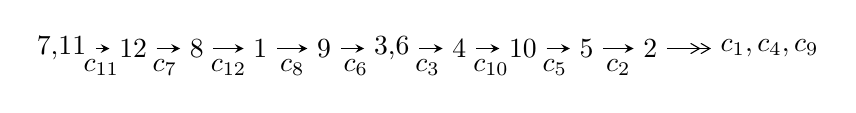
\begin{tikzpicture}[x=23pt, y=7pt]
	% node
	\node (A0) at (-1/8, 0) {7,11};
	\node (A1) at (1, 0) {12};
	\node (A2) at (2, 0) {8};
	\node (A3) at (3, 0) {1};
	\node (A4) at (4, 0) {9};
	\node (A5) at (81/16, 0) {3,6};
	\node (A6) at (49/8, 0) {4};
	\node (A7) at (57/8, 0) {10};
	\node (A8) at (65/8, 0) {5};
	\node (A9) at (73/8, 0) {2};
	\node (C1) at (1/2, -1) {$c_{11}$};
	\node (C2) at (3/2, -1) {$c_{7}$};
	\node (C3) at (5/2, -1) {$c_{12}$};
	\node (C4) at (7/2, -1) {$c_{8}$};
	\node (C5) at (9/2, -1) {$c_{6}$};
	\node (C6) at (45/8, -1) {$c_{3}$};
	\node (C7) at (53/8, -1) {$c_{10}$};
	\node (C8) at (61/8, -1) {$c_{5}$};
	\node (C9) at (69/8, -1) {$c_{2}$};
	\node (A10) at (11, 0) {$c_{1},c_{4},c_{9}$};

	% edge
	\draw[->,>=stealth]	
	(A0) edge (A1) (A1) edge (A2) (A2) edge (A3) (A3) edge (A4) (A4) edge (A5) (A5) edge (A6) (A6) edge (A7) (A7) edge (A8) (A8) edge (A9) ;
	\draw[->>,>={angle 60}]	
	(A9) edge (A10);
\end{tikzpicture} \\ 

\end{tabular} \\

\footnotetext{
The image of knot diagram is generated by the software ``\textbf{Draw programme}" developed by Andrew Bartholomew(\url{http://www.layer8.co.uk/maths/draw/index.htm\#Running-draw}), where we modified some parts for our purpose(\url{https://github.com/CATsTAILs/LinksPainter}).
}\phantom \\ \newline 
\centering \textbf{Ideals for irreducible components\footnotemark of $X_{\text{par}}$} 
 
\begin{align*}
I^u_{1}&=\langle 
-437 u^{29}+1525 u^{28}+\cdots+13 b+2231,\;5117 u^{29}-17060 u^{28}+\cdots+143 a-29622,\\
\phantom{I^u_{1}}&\phantom{= \langle  }u^{30}-5 u^{29}+\cdots-38 u+11\rangle \\
I^u_{2}&=\langle 
-269 u^{22} a+526 u^{22}+\cdots-286 a-712,\;2 u^{22} a+3 u^{22}+\cdots-7 a-6,\;u^{23}+2 u^{22}+\cdots-2 u+1\rangle \\
I^u_{3}&=\langle 
u^8- u^7-5 u^6+5 u^5+7 u^4-6 u^3-4 u^2+b+2 u,\;- u^2+a+2,\\
\phantom{I^u_{3}}&\phantom{= \langle  }u^9-2 u^8-5 u^7+11 u^6+6 u^5-17 u^4- u^3+8 u^2- u+1\rangle \\
I^u_{4}&=\langle 
b+a- u-1,\;a^2-3 a u-2 a+u+2,\;u^2+u-1\rangle \\
\\
I^v_{1}&=\langle 
a,\;b-1,\;v+1\rangle \\
\end{align*}
\raggedright * 5 irreducible components of $\dim_{\mathbb{C}}=0$, with total 90 representations.\\
\footnotetext{All coefficients of polynomials are rational numbers. But the coefficients are sometimes approximated in decimal forms when there is not enough margin.}
\newpage
\renewcommand{\arraystretch}{1}
\centering \section*{I. $I^u_{1}= \langle -437 u^{29}+1525 u^{28}+\cdots+13 b+2231,\;5117 u^{29}-17060 u^{28}+\cdots+143 a-29622,\;u^{30}-5 u^{29}+\cdots-38 u+11 \rangle$}
\flushleft \textbf{(i) Arc colorings}\\
\begin{tabular}{m{7pt} m{180pt} m{7pt} m{180pt} }
\flushright $a_{7}=$&$\begin{pmatrix}0\\u\end{pmatrix}$ \\
\flushright $a_{11}=$&$\begin{pmatrix}1\\0\end{pmatrix}$ \\
\flushright $a_{12}=$&$\begin{pmatrix}1\\- u^2\end{pmatrix}$ \\
\flushright $a_{8}=$&$\begin{pmatrix}u\\- u^3+u\end{pmatrix}$ \\
\flushright $a_{1}=$&$\begin{pmatrix}- u^2+1\\u^4-2 u^2\end{pmatrix}$ \\
\flushright $a_{9}=$&$\begin{pmatrix}- u^3+2 u\\u^5-3 u^3+u\end{pmatrix}$ \\
\flushright $a_{3}=$&$\begin{pmatrix}-35.7832 u^{29}+119.301 u^{28}+\cdots-569.783 u+207.147\\33.6154 u^{29}-117.308 u^{28}+\cdots+442.615 u-171.615\end{pmatrix}$ \\
\flushright $a_{6}=$&$\begin{pmatrix}- u\\u\end{pmatrix}$ \\
\flushright $a_{4}=$&$\begin{pmatrix}-21.4755 u^{29}+79.1469 u^{28}+\cdots-257.476 u+109.839\\19.3077 u^{29}-77.1538 u^{28}+\cdots+130.308 u-74.3077\end{pmatrix}$ \\
\flushright $a_{10}=$&$\begin{pmatrix}-11.2448 u^{29}+33.5315 u^{28}+\cdots-296.245 u+97.6084\\21.6923 u^{29}-63.8462 u^{28}+\cdots+601.692 u-187.692\end{pmatrix}$ \\
\flushright $a_{5}=$&$\begin{pmatrix}27.0629 u^{29}-88.6224 u^{28}+\cdots+448.063 u-156.699\\-12.5385 u^{29}+34.7692 u^{28}+\cdots-371.538 u+113.538\end{pmatrix}$ \\
\flushright $a_{2}=$&$\begin{pmatrix}-28.1678 u^{29}+95.9930 u^{28}+\cdots-426.168 u+161.531\\33.4615 u^{29}-116.231 u^{28}+\cdots+484.462 u-183.462\end{pmatrix}$\\&\end{tabular}
\flushleft \textbf{(ii) Obstruction class $= -1$}\\~\\
\flushleft \textbf{(iii) Cusp Shapes $= \frac{697}{13} u^{29}-\frac{2097}{13} u^{28}+\cdots+\frac{18078}{13} u-\frac{5897}{13}$}\\~\\
\newpage\renewcommand{\arraystretch}{1}
\flushleft \textbf{(iv) u-Polynomials at the component}\newline \\
\begin{tabular}{m{50pt}|m{274pt}}
Crossings & \hspace{64pt}u-Polynomials at each crossing \\
\hline $$\begin{aligned}c_{1},c_{3}\end{aligned}$$&$\begin{aligned}
&u^{30}+4 u^{29}+\cdots+5 u-1
\end{aligned}$\\
\hline $$\begin{aligned}c_{2}\end{aligned}$$&$\begin{aligned}
&u^{30}+17 u^{29}+\cdots-21 u-11
\end{aligned}$\\
\hline $$\begin{aligned}c_{4},c_{10}\end{aligned}$$&$\begin{aligned}
&u^{30}-6 u^{28}+\cdots-3 u-1
\end{aligned}$\\
\hline $$\begin{aligned}c_{5},c_{9}\end{aligned}$$&$\begin{aligned}
&u^{30}- u^{29}+\cdots-4 u+1
\end{aligned}$\\
\hline $$\begin{aligned}c_{6},c_{7},c_{8}\\c_{11},c_{12}\end{aligned}$$&$\begin{aligned}
&u^{30}+5 u^{29}+\cdots+38 u+11
\end{aligned}$\\
\hline
\end{tabular}\\~\\
\newpage\renewcommand{\arraystretch}{1}
\flushleft \textbf{(v) Riley Polynomials at the component}\newline \\
\begin{tabular}{m{50pt}|m{274pt}}
Crossings & \hspace{64pt}Riley Polynomials at each crossing \\
\hline $$\begin{aligned}c_{1},c_{3}\end{aligned}$$&$\begin{aligned}
&y^{30}+28 y^{28}+\cdots-93 y+1
\end{aligned}$\\
\hline $$\begin{aligned}c_{2}\end{aligned}$$&$\begin{aligned}
&y^{30}-3 y^{29}+\cdots-1739 y+121
\end{aligned}$\\
\hline $$\begin{aligned}c_{4},c_{10}\end{aligned}$$&$\begin{aligned}
&y^{30}-12 y^{29}+\cdots-33 y+1
\end{aligned}$\\
\hline $$\begin{aligned}c_{5},c_{9}\end{aligned}$$&$\begin{aligned}
&y^{30}-19 y^{29}+\cdots-38 y+1
\end{aligned}$\\
\hline $$\begin{aligned}c_{6},c_{7},c_{8}\\c_{11},c_{12}\end{aligned}$$&$\begin{aligned}
&y^{30}-43 y^{29}+\cdots-1180 y+121
\end{aligned}$\\
\hline
\end{tabular}\\~\\
\newpage\flushleft \textbf{(vi) Complex Volumes and Cusp Shapes}
$$\begin{array}{c|c|c}  
\text{Solutions to }I^u_{1}& \I (\text{vol} + \sqrt{-1}CS) & \text{Cusp shape}\\
 \hline 
\begin{aligned}
u &= \phantom{-}1.01658\phantom{ +0.000000I} \\
a &= \phantom{-}2.92862\phantom{ +0.000000I} \\
b &= -1.50043\phantom{ +0.000000I}\end{aligned}
 & \phantom{-}1.74384\phantom{ +0.000000I} & \phantom{-}5.98900\phantom{ +0.000000I} \\ \hline\begin{aligned}
u &= -0.878022 + 0.002899 I \\
a &= \phantom{-}0.238285 + 0.304913 I \\
b &= -0.559876 - 0.690935 I\end{aligned}
 & \phantom{-}1.314950 - 0.451834 I & \phantom{-}6.61404 + 1.58489 I \\ \hline\begin{aligned}
u &= -0.878022 - 0.002899 I \\
a &= \phantom{-}0.238285 - 0.304913 I \\
b &= -0.559876 + 0.690935 I\end{aligned}
 & \phantom{-}1.314950 + 0.451834 I & \phantom{-}6.61404 - 1.58489 I \\ \hline\begin{aligned}
u &= -1.130260 + 0.186589 I \\
a &= -1.246950 - 0.354613 I \\
b &= \phantom{-}0.627496 - 0.880698 I\end{aligned}
 & \phantom{-}3.04303 - 4.92292 I & \phantom{-}3.35262 + 6.51542 I \\ \hline\begin{aligned}
u &= -1.130260 - 0.186589 I \\
a &= -1.246950 + 0.354613 I \\
b &= \phantom{-}0.627496 + 0.880698 I\end{aligned}
 & \phantom{-}3.04303 + 4.92292 I & \phantom{-}3.35262 - 6.51542 I \\ \hline\begin{aligned}
u &= \phantom{-}1.18652\phantom{ +0.000000I} \\
a &= -1.61412\phantom{ +0.000000I} \\
b &= \phantom{-}1.01453\phantom{ +0.000000I}\end{aligned}
 & \phantom{-}6.25305\phantom{ +0.000000I} & \phantom{-}14.0800\phantom{ +0.000000I} \\ \hline\begin{aligned}
u &= \phantom{-}0.313981 + 0.719655 I \\
a &= -0.258210 - 0.371938 I \\
b &= -0.865351 + 0.635662 I\end{aligned}
 & \phantom{-}0.07877 - 5.69968 I & \phantom{-}6.25097 + 7.15473 I \\ \hline\begin{aligned}
u &= \phantom{-}0.313981 - 0.719655 I \\
a &= -0.258210 + 0.371938 I \\
b &= -0.865351 - 0.635662 I\end{aligned}
 & \phantom{-}0.07877 + 5.69968 I & \phantom{-}6.25097 - 7.15473 I \\ \hline\begin{aligned}
u &= \phantom{-}0.439811 + 0.644843 I \\
a &= -0.712132 + 0.794843 I \\
b &= \phantom{-}1.079900 + 0.783683 I\end{aligned}
 & \phantom{-}0.48551 + 10.07530 I & \phantom{-}5.95949 - 9.67797 I \\ \hline\begin{aligned}
u &= \phantom{-}0.439811 - 0.644843 I \\
a &= -0.712132 - 0.794843 I \\
b &= \phantom{-}1.079900 - 0.783683 I\end{aligned}
 & \phantom{-}0.48551 - 10.07530 I & \phantom{-}5.95949 + 9.67797 I\\
 \hline 
 \end{array}$$\newpage$$\begin{array}{c|c|c}  
\text{Solutions to }I^u_{1}& \I (\text{vol} + \sqrt{-1}CS) & \text{Cusp shape}\\
 \hline 
\begin{aligned}
u &= -1.174900 + 0.352174 I \\
a &= \phantom{-}1.84786 + 0.33394 I \\
b &= -1.28819 + 0.84300 I\end{aligned}
 & \phantom{-}5.5646 - 13.4956 I & \phantom{-}9.26736 + 8.87328 I \\ \hline\begin{aligned}
u &= -1.174900 - 0.352174 I \\
a &= \phantom{-}1.84786 - 0.33394 I \\
b &= -1.28819 - 0.84300 I\end{aligned}
 & \phantom{-}5.5646 + 13.4956 I & \phantom{-}9.26736 - 8.87328 I \\ \hline\begin{aligned}
u &= -1.198660 + 0.506727 I \\
a &= -0.495699 - 0.735221 I \\
b &= \phantom{-}0.712841 + 0.295117 I\end{aligned}
 & \phantom{-}4.63959 + 1.45693 I & \phantom{-}20.4781 - 6.0794 I \\ \hline\begin{aligned}
u &= -1.198660 - 0.506727 I \\
a &= -0.495699 + 0.735221 I \\
b &= \phantom{-}0.712841 - 0.295117 I\end{aligned}
 & \phantom{-}4.63959 - 1.45693 I & \phantom{-}20.4781 + 6.0794 I \\ \hline\begin{aligned}
u &= -1.32795\phantom{ +0.000000I} \\
a &= -0.917911\phantom{ +0.000000I} \\
b &= \phantom{-}0.203761\phantom{ +0.000000I}\end{aligned}
 & \phantom{-}3.16863\phantom{ +0.000000I} & \phantom{-}1.59560\phantom{ +0.000000I} \\ \hline\begin{aligned}
u &= \phantom{-}0.360310 + 0.392975 I \\
a &= \phantom{-}0.55572 - 1.55779 I \\
b &= -0.494454 - 0.710271 I\end{aligned}
 & -1.69300 + 2.96011 I & -0.46924 - 8.93785 I \\ \hline\begin{aligned}
u &= \phantom{-}0.360310 - 0.392975 I \\
a &= \phantom{-}0.55572 + 1.55779 I \\
b &= -0.494454 + 0.710271 I\end{aligned}
 & -1.69300 - 2.96011 I & -0.46924 + 8.93785 I \\ \hline\begin{aligned}
u &= -0.481507\phantom{ +0.000000I} \\
a &= \phantom{-}0.778558\phantom{ +0.000000I} \\
b &= -0.569296\phantom{ +0.000000I}\end{aligned}
 & \phantom{-}0.855934\phantom{ +0.000000I} & \phantom{-}11.6870\phantom{ +0.000000I} \\ \hline\begin{aligned}
u &= \phantom{-}0.270687 + 0.323054 I \\
a &= \phantom{-}1.45188 - 0.61952 I \\
b &= \phantom{-}0.413056 - 0.459484 I\end{aligned}
 & -1.90583 - 0.45249 I & -1.79458 - 1.14821 I \\ \hline\begin{aligned}
u &= \phantom{-}0.270687 - 0.323054 I \\
a &= \phantom{-}1.45188 + 0.61952 I \\
b &= \phantom{-}0.413056 + 0.459484 I\end{aligned}
 & -1.90583 + 0.45249 I & -1.79458 + 1.14821 I\\
 \hline 
 \end{array}$$\newpage$$\begin{array}{c|c|c}  
\text{Solutions to }I^u_{1}& \I (\text{vol} + \sqrt{-1}CS) & \text{Cusp shape}\\
 \hline 
\begin{aligned}
u &= \phantom{-}1.70982 + 0.01754 I \\
a &= -0.504443 - 0.628284 I \\
b &= \phantom{-}0.562401 + 1.059590 I\end{aligned}
 & \phantom{-}10.64730 - 0.25494 I & \phantom{-0.000000 } 0 \\ \hline\begin{aligned}
u &= \phantom{-}1.70982 - 0.01754 I \\
a &= -0.504443 + 0.628284 I \\
b &= \phantom{-}0.562401 - 1.059590 I\end{aligned}
 & \phantom{-}10.64730 + 0.25494 I & \phantom{-0.000000 } 0 \\ \hline\begin{aligned}
u &= -1.73772\phantom{ +0.000000I} \\
a &= -2.71628\phantom{ +0.000000I} \\
b &= \phantom{-}1.72980\phantom{ +0.000000I}\end{aligned}
 & \phantom{-}11.7131\phantom{ +0.000000I} & \phantom{-0.000000 } 0 \\ \hline\begin{aligned}
u &= \phantom{-}1.76484 + 0.04602 I \\
a &= \phantom{-}1.241500 + 0.064835 I \\
b &= -0.701863 - 0.995930 I\end{aligned}
 & \phantom{-}13.5460 + 5.9087 I & \phantom{-0.000000 } 0 \\ \hline\begin{aligned}
u &= \phantom{-}1.76484 - 0.04602 I \\
a &= \phantom{-}1.241500 - 0.064835 I \\
b &= -0.701863 + 0.995930 I\end{aligned}
 & \phantom{-}13.5460 - 5.9087 I & \phantom{-0.000000 } 0 \\ \hline\begin{aligned}
u &= \phantom{-}1.77253 + 0.09377 I \\
a &= -2.08526 - 0.07253 I \\
b &= \phantom{-}1.43463 + 0.88148 I\end{aligned}
 & \phantom{-}16.1500 + 15.4410 I & \phantom{-0.000000 } 0 \\ \hline\begin{aligned}
u &= \phantom{-}1.77253 - 0.09377 I \\
a &= -2.08526 + 0.07253 I \\
b &= \phantom{-}1.43463 - 0.88148 I\end{aligned}
 & \phantom{-}16.1500 - 15.4410 I & \phantom{-0.000000 } 0 \\ \hline\begin{aligned}
u &= -1.77800\phantom{ +0.000000I} \\
a &= \phantom{-}1.81911\phantom{ +0.000000I} \\
b &= -1.19344\phantom{ +0.000000I}\end{aligned}
 & \phantom{-}17.0939\phantom{ +0.000000I} & \phantom{-0.000000 } 0 \\ \hline\begin{aligned}
u &= \phantom{-}1.81090 + 0.09745 I \\
a &= \phantom{-}1.055730 - 0.361250 I \\
b &= -0.763050 - 0.096600 I\end{aligned}
 & \phantom{-}15.7188 + 1.2036 I & \phantom{-0.000000 } 0 \\ \hline\begin{aligned}
u &= \phantom{-}1.81090 - 0.09745 I \\
a &= \phantom{-}1.055730 + 0.361250 I \\
b &= -0.763050 + 0.096600 I\end{aligned}
 & \phantom{-}15.7188 - 1.2036 I & \phantom{-0.000000 } 0\\
 \hline 
 \end{array}$$\newpage\newpage\renewcommand{\arraystretch}{1}
\centering \section*{II. $I^u_{2}= \langle -269 u^{22} a+526 u^{22}+\cdots-286 a-712,\;2 u^{22} a+3 u^{22}+\cdots-7 a-6,\;u^{23}+2 u^{22}+\cdots-2 u+1 \rangle$}
\flushleft \textbf{(i) Arc colorings}\\
\begin{tabular}{m{7pt} m{180pt} m{7pt} m{180pt} }
\flushright $a_{7}=$&$\begin{pmatrix}0\\u\end{pmatrix}$ \\
\flushright $a_{11}=$&$\begin{pmatrix}1\\0\end{pmatrix}$ \\
\flushright $a_{12}=$&$\begin{pmatrix}1\\- u^2\end{pmatrix}$ \\
\flushright $a_{8}=$&$\begin{pmatrix}u\\- u^3+u\end{pmatrix}$ \\
\flushright $a_{1}=$&$\begin{pmatrix}- u^2+1\\u^4-2 u^2\end{pmatrix}$ \\
\flushright $a_{9}=$&$\begin{pmatrix}- u^3+2 u\\u^5-3 u^3+u\end{pmatrix}$ \\
\flushright $a_{3}=$&$\begin{pmatrix}a\\0.651332 a u^{22}-1.27361 u^{22}+\cdots+0.692494 a+1.72397\end{pmatrix}$ \\
\flushright $a_{6}=$&$\begin{pmatrix}- u\\u\end{pmatrix}$ \\
\flushright $a_{4}=$&$\begin{pmatrix}-2.45521 a u^{22}+1.61501 u^{22}+\cdots-0.707022 a+0.806295\\3.10654 a u^{22}-2.88862 u^{22}+\cdots+2.39952 a+0.917676\end{pmatrix}$ \\
\flushright $a_{10}=$&$\begin{pmatrix}0.273608 a u^{22}-0.486683 u^{22}+\cdots-1.72397 a-0.0750605\\0.00726392 a u^{22}+2.23487 u^{22}+\cdots-0.222760 a-1.86925\end{pmatrix}$ \\
\flushright $a_{5}=$&$\begin{pmatrix}-1.01453 a u^{22}+1.53027 u^{22}+\cdots+0.445521 a+1.73850\\1.44068 a u^{22}-4.08475 u^{22}+\cdots+1.15254 a+0.932203\end{pmatrix}$ \\
\flushright $a_{2}=$&$\begin{pmatrix}0.806295 a u^{22}-3.92978 u^{22}+\cdots+1.27361 a-2.48668\\-0.806295 a u^{22}+4.92978 u^{22}+\cdots-1.27361 a+0.486683\end{pmatrix}$\\&\end{tabular}
\flushleft \textbf{(ii) Obstruction class $= -1$}\\~\\
\flushleft \textbf{(iii) Cusp Shapes $= u^{22}-10 u^{21}-25 u^{20}+139 u^{19}+224 u^{18}-798 u^{17}-1029 u^{16}+2424 u^{15}+2796 u^{14}-4094 u^{13}-4866 u^{12}+3507 u^{11}+5634 u^{10}-630 u^9-4167 u^8-1372 u^7+1603 u^6+1148 u^5-81 u^4-337 u^3-100 u^2+12 u+27$}\\~\\
\newpage\renewcommand{\arraystretch}{1}
\flushleft \textbf{(iv) u-Polynomials at the component}\newline \\
\begin{tabular}{m{50pt}|m{274pt}}
Crossings & \hspace{64pt}u-Polynomials at each crossing \\
\hline $$\begin{aligned}c_{1},c_{3}\end{aligned}$$&$\begin{aligned}
&u^{46}-5 u^{45}+\cdots+602 u-47
\end{aligned}$\\
\hline $$\begin{aligned}c_{2}\end{aligned}$$&$\begin{aligned}
&(u^{23}-11 u^{22}+\cdots+14 u-4)^{2}
\end{aligned}$\\
\hline $$\begin{aligned}c_{4},c_{10}\end{aligned}$$&$\begin{aligned}
&u^{46}-8 u^{44}+\cdots+2009 u+851
\end{aligned}$\\
\hline $$\begin{aligned}c_{5},c_{9}\end{aligned}$$&$\begin{aligned}
&u^{46}+2 u^{44}+\cdots- u-1
\end{aligned}$\\
\hline $$\begin{aligned}c_{6},c_{7},c_{8}\\c_{11},c_{12}\end{aligned}$$&$\begin{aligned}
&(u^{23}-2 u^{22}+\cdots-2 u-1)^{2}
\end{aligned}$\\
\hline
\end{tabular}\\~\\
\newpage\renewcommand{\arraystretch}{1}
\flushleft \textbf{(v) Riley Polynomials at the component}\newline \\
\begin{tabular}{m{50pt}|m{274pt}}
Crossings & \hspace{64pt}Riley Polynomials at each crossing \\
\hline $$\begin{aligned}c_{1},c_{3}\end{aligned}$$&$\begin{aligned}
&y^{46}+23 y^{45}+\cdots-6896 y+2209
\end{aligned}$\\
\hline $$\begin{aligned}c_{2}\end{aligned}$$&$\begin{aligned}
&(y^{23}-5 y^{22}+\cdots+268 y-16)^{2}
\end{aligned}$\\
\hline $$\begin{aligned}c_{4},c_{10}\end{aligned}$$&$\begin{aligned}
&y^{46}-16 y^{45}+\cdots-19209411 y+724201
\end{aligned}$\\
\hline $$\begin{aligned}c_{5},c_{9}\end{aligned}$$&$\begin{aligned}
&y^{46}+4 y^{45}+\cdots-35 y+1
\end{aligned}$\\
\hline $$\begin{aligned}c_{6},c_{7},c_{8}\\c_{11},c_{12}\end{aligned}$$&$\begin{aligned}
&(y^{23}-32 y^{22}+\cdots+18 y-1)^{2}
\end{aligned}$\\
\hline
\end{tabular}\\~\\
\newpage\flushleft \textbf{(vi) Complex Volumes and Cusp Shapes}
$$\begin{array}{c|c|c}  
\text{Solutions to }I^u_{2}& \I (\text{vol} + \sqrt{-1}CS) & \text{Cusp shape}\\
 \hline 
\begin{aligned}
u &= \phantom{-}0.999683 + 0.186821 I \\
a &= -0.042700 - 1.410890 I \\
b &= -0.18371 + 1.64920 I\end{aligned}
 & \phantom{-}2.50463 + 5.52558 I & \phantom{-}5.10396 - 8.15770 I \\ \hline\begin{aligned}
u &= \phantom{-}0.999683 + 0.186821 I \\
a &= \phantom{-}1.68330 - 1.01369 I \\
b &= -0.995212 - 0.632466 I\end{aligned}
 & \phantom{-}2.50463 + 5.52558 I & \phantom{-}5.10396 - 8.15770 I \\ \hline\begin{aligned}
u &= \phantom{-}0.999683 - 0.186821 I \\
a &= -0.042700 + 1.410890 I \\
b &= -0.18371 - 1.64920 I\end{aligned}
 & \phantom{-}2.50463 - 5.52558 I & \phantom{-}5.10396 + 8.15770 I \\ \hline\begin{aligned}
u &= \phantom{-}0.999683 - 0.186821 I \\
a &= \phantom{-}1.68330 + 1.01369 I \\
b &= -0.995212 + 0.632466 I\end{aligned}
 & \phantom{-}2.50463 - 5.52558 I & \phantom{-}5.10396 + 8.15770 I \\ \hline\begin{aligned}
u &= -1.105860 + 0.055480 I \\
a &= -1.92578 + 0.18458 I \\
b &= \phantom{-}1.35825 - 1.09576 I\end{aligned}
 & \phantom{-}5.84113 - 4.35667 I & \phantom{-}13.8335 + 5.4983 I \\ \hline\begin{aligned}
u &= -1.105860 + 0.055480 I \\
a &= \phantom{-}1.60049 - 1.41054 I \\
b &= -0.614170 - 0.043824 I\end{aligned}
 & \phantom{-}5.84113 - 4.35667 I & \phantom{-}13.8335 + 5.4983 I \\ \hline\begin{aligned}
u &= -1.105860 - 0.055480 I \\
a &= -1.92578 - 0.18458 I \\
b &= \phantom{-}1.35825 + 1.09576 I\end{aligned}
 & \phantom{-}5.84113 + 4.35667 I & \phantom{-}13.8335 - 5.4983 I \\ \hline\begin{aligned}
u &= -1.105860 - 0.055480 I \\
a &= \phantom{-}1.60049 + 1.41054 I \\
b &= -0.614170 + 0.043824 I\end{aligned}
 & \phantom{-}5.84113 + 4.35667 I & \phantom{-}13.8335 - 5.4983 I \\ \hline\begin{aligned}
u &= \phantom{-}1.18981\phantom{ +0.000000I} \\
a &= -1.50802\phantom{ +0.000000I} \\
b &= \phantom{-}1.05229\phantom{ +0.000000I}\end{aligned}
 & \phantom{-}6.25240\phantom{ +0.000000I} & \phantom{-}14.1390\phantom{ +0.000000I} \\ \hline\begin{aligned}
u &= \phantom{-}1.18981\phantom{ +0.000000I} \\
a &= -1.73509\phantom{ +0.000000I} \\
b &= \phantom{-}0.992937\phantom{ +0.000000I}\end{aligned}
 & \phantom{-}6.25240\phantom{ +0.000000I} & \phantom{-}14.1390\phantom{ +0.000000I}\\
 \hline 
 \end{array}$$\newpage$$\begin{array}{c|c|c}  
\text{Solutions to }I^u_{2}& \I (\text{vol} + \sqrt{-1}CS) & \text{Cusp shape}\\
 \hline 
\begin{aligned}
u &= \phantom{-}1.140950 + 0.349828 I \\
a &= \phantom{-}0.851056 - 0.861201 I \\
b &= -0.901717 - 0.147878 I\end{aligned}
 & \phantom{-}7.12094 + 5.39909 I & \phantom{-}13.5404 - 6.0968 I \\ \hline\begin{aligned}
u &= \phantom{-}1.140950 + 0.349828 I \\
a &= -1.70952 + 0.17931 I \\
b &= \phantom{-}1.30005 + 0.76522 I\end{aligned}
 & \phantom{-}7.12094 + 5.39909 I & \phantom{-}13.5404 - 6.0968 I \\ \hline\begin{aligned}
u &= \phantom{-}1.140950 - 0.349828 I \\
a &= \phantom{-}0.851056 + 0.861201 I \\
b &= -0.901717 + 0.147878 I\end{aligned}
 & \phantom{-}7.12094 - 5.39909 I & \phantom{-}13.5404 + 6.0968 I \\ \hline\begin{aligned}
u &= \phantom{-}1.140950 - 0.349828 I \\
a &= -1.70952 - 0.17931 I \\
b &= \phantom{-}1.30005 - 0.76522 I\end{aligned}
 & \phantom{-}7.12094 - 5.39909 I & \phantom{-}13.5404 + 6.0968 I \\ \hline\begin{aligned}
u &= -0.377702 + 0.629512 I \\
a &= \phantom{-}0.209564 - 0.786199 I \\
b &= \phantom{-}0.780693 + 0.190315 I\end{aligned}
 & \phantom{-}2.35417 - 2.04864 I & \phantom{-}12.02442 + 4.27551 I \\ \hline\begin{aligned}
u &= -0.377702 + 0.629512 I \\
a &= \phantom{-}0.341684 + 0.460205 I \\
b &= -0.932101 + 0.597740 I\end{aligned}
 & \phantom{-}2.35417 - 2.04864 I & \phantom{-}12.02442 + 4.27551 I \\ \hline\begin{aligned}
u &= -0.377702 - 0.629512 I \\
a &= \phantom{-}0.209564 + 0.786199 I \\
b &= \phantom{-}0.780693 - 0.190315 I\end{aligned}
 & \phantom{-}2.35417 + 2.04864 I & \phantom{-}12.02442 - 4.27551 I \\ \hline\begin{aligned}
u &= -0.377702 - 0.629512 I \\
a &= \phantom{-}0.341684 - 0.460205 I \\
b &= -0.932101 - 0.597740 I\end{aligned}
 & \phantom{-}2.35417 + 2.04864 I & \phantom{-}12.02442 - 4.27551 I \\ \hline\begin{aligned}
u &= -0.580448 + 0.322591 I \\
a &= -0.345114 + 0.640960 I \\
b &= -0.861693 - 0.321506 I\end{aligned}
 & \phantom{-}0.229739 + 0.719364 I & \phantom{-}7.70501 - 1.54064 I \\ \hline\begin{aligned}
u &= -0.580448 + 0.322591 I \\
a &= \phantom{-}2.10527 + 0.09680 I \\
b &= -0.966346 + 0.634688 I\end{aligned}
 & \phantom{-}0.229739 + 0.719364 I & \phantom{-}7.70501 - 1.54064 I\\
 \hline 
 \end{array}$$\newpage$$\begin{array}{c|c|c}  
\text{Solutions to }I^u_{2}& \I (\text{vol} + \sqrt{-1}CS) & \text{Cusp shape}\\
 \hline 
\begin{aligned}
u &= -0.580448 - 0.322591 I \\
a &= -0.345114 - 0.640960 I \\
b &= -0.861693 + 0.321506 I\end{aligned}
 & \phantom{-}0.229739 - 0.719364 I & \phantom{-}7.70501 + 1.54064 I \\ \hline\begin{aligned}
u &= -0.580448 - 0.322591 I \\
a &= \phantom{-}2.10527 - 0.09680 I \\
b &= -0.966346 - 0.634688 I\end{aligned}
 & \phantom{-}0.229739 - 0.719364 I & \phantom{-}7.70501 + 1.54064 I \\ \hline\begin{aligned}
u &= -0.157596 + 0.449298 I \\
a &= \phantom{-}0.51417 - 1.77331 I \\
b &= \phantom{-}0.893978 - 0.534579 I\end{aligned}
 & -1.03877 - 3.41304 I & -1.13516 + 7.69580 I \\ \hline\begin{aligned}
u &= -0.157596 + 0.449298 I \\
a &= -0.0565579 + 0.1078630 I \\
b &= \phantom{-}0.545955 + 1.142730 I\end{aligned}
 & -1.03877 - 3.41304 I & -1.13516 + 7.69580 I \\ \hline\begin{aligned}
u &= -0.157596 - 0.449298 I \\
a &= \phantom{-}0.51417 + 1.77331 I \\
b &= \phantom{-}0.893978 + 0.534579 I\end{aligned}
 & -1.03877 + 3.41304 I & -1.13516 - 7.69580 I \\ \hline\begin{aligned}
u &= -0.157596 - 0.449298 I \\
a &= -0.0565579 - 0.1078630 I \\
b &= \phantom{-}0.545955 - 1.142730 I\end{aligned}
 & -1.03877 + 3.41304 I & -1.13516 - 7.69580 I \\ \hline\begin{aligned}
u &= \phantom{-}1.59673\phantom{ +0.000000I} \\
a &= -0.0933260\phantom{ +0.000000I} \\
b &= \phantom{-}0.587557\phantom{ +0.000000I}\end{aligned}
 & \phantom{-}7.42882\phantom{ +0.000000I} & \phantom{-}28.8540\phantom{ +0.000000I} \\ \hline\begin{aligned}
u &= \phantom{-}1.59673\phantom{ +0.000000I} \\
a &= -2.54753\phantom{ +0.000000I} \\
b &= \phantom{-}1.94206\phantom{ +0.000000I}\end{aligned}
 & \phantom{-}7.42882\phantom{ +0.000000I} & \phantom{-}28.8540\phantom{ +0.000000I} \\ \hline\begin{aligned}
u &= \phantom{-}0.313095 + 0.086295 I \\
a &= \phantom{-}1.18015 - 2.03047 I \\
b &= -0.959828 - 0.907570 I\end{aligned}
 & \phantom{-}1.29868 + 3.82978 I & \phantom{-}14.5236 - 8.4853 I \\ \hline\begin{aligned}
u &= \phantom{-}0.313095 + 0.086295 I \\
a &= -2.82861 - 3.70039 I \\
b &= \phantom{-}0.569721 + 0.399803 I\end{aligned}
 & \phantom{-}1.29868 + 3.82978 I & \phantom{-}14.5236 - 8.4853 I\\
 \hline 
 \end{array}$$\newpage$$\begin{array}{c|c|c}  
\text{Solutions to }I^u_{2}& \I (\text{vol} + \sqrt{-1}CS) & \text{Cusp shape}\\
 \hline 
\begin{aligned}
u &= \phantom{-}0.313095 - 0.086295 I \\
a &= \phantom{-}1.18015 + 2.03047 I \\
b &= -0.959828 + 0.907570 I\end{aligned}
 & \phantom{-}1.29868 - 3.82978 I & \phantom{-}14.5236 + 8.4853 I \\ \hline\begin{aligned}
u &= \phantom{-}0.313095 - 0.086295 I \\
a &= -2.82861 + 3.70039 I \\
b &= \phantom{-}0.569721 - 0.399803 I\end{aligned}
 & \phantom{-}1.29868 - 3.82978 I & \phantom{-}14.5236 + 8.4853 I \\ \hline\begin{aligned}
u &= -1.73349 + 0.04283 I \\
a &= -0.05422 - 1.72140 I \\
b &= \phantom{-}0.12177 + 1.99221 I\end{aligned}
 & \phantom{-}12.35220 - 6.42236 I & \phantom{-}6.09016 + 6.34054 I \\ \hline\begin{aligned}
u &= -1.73349 + 0.04283 I \\
a &= -1.78344 - 0.36813 I \\
b &= \phantom{-}1.091730 - 0.703323 I\end{aligned}
 & \phantom{-}12.35220 - 6.42236 I & \phantom{-}6.09016 + 6.34054 I \\ \hline\begin{aligned}
u &= -1.73349 - 0.04283 I \\
a &= -0.05422 + 1.72140 I \\
b &= \phantom{-}0.12177 - 1.99221 I\end{aligned}
 & \phantom{-}12.35220 + 6.42236 I & \phantom{-}6.09016 - 6.34054 I \\ \hline\begin{aligned}
u &= -1.73349 - 0.04283 I \\
a &= -1.78344 + 0.36813 I \\
b &= \phantom{-}1.091730 + 0.703323 I\end{aligned}
 & \phantom{-}12.35220 + 6.42236 I & \phantom{-}6.09016 - 6.34054 I \\ \hline\begin{aligned}
u &= \phantom{-}1.75724 + 0.01445 I \\
a &= -1.45201 - 0.83740 I \\
b &= \phantom{-}0.696220 - 0.251137 I\end{aligned}
 & \phantom{-}16.2384 + 4.6560 I & \phantom{-}13.26850 - 4.63684 I \\ \hline\begin{aligned}
u &= \phantom{-}1.75724 + 0.01445 I \\
a &= \phantom{-}2.07313 + 0.57426 I \\
b &= -1.57300 - 1.18808 I\end{aligned}
 & \phantom{-}16.2384 + 4.6560 I & \phantom{-}13.26850 - 4.63684 I \\ \hline\begin{aligned}
u &= \phantom{-}1.75724 - 0.01445 I \\
a &= -1.45201 + 0.83740 I \\
b &= \phantom{-}0.696220 + 0.251137 I\end{aligned}
 & \phantom{-}16.2384 - 4.6560 I & \phantom{-}13.26850 + 4.63684 I \\ \hline\begin{aligned}
u &= \phantom{-}1.75724 - 0.01445 I \\
a &= \phantom{-}2.07313 - 0.57426 I \\
b &= -1.57300 + 1.18808 I\end{aligned}
 & \phantom{-}16.2384 - 4.6560 I & \phantom{-}13.26850 + 4.63684 I\\
 \hline 
 \end{array}$$\newpage$$\begin{array}{c|c|c}  
\text{Solutions to }I^u_{2}& \I (\text{vol} + \sqrt{-1}CS) & \text{Cusp shape}\\
 \hline 
\begin{aligned}
u &= -1.76372 + 0.09254 I \\
a &= -1.227110 - 0.467441 I \\
b &= \phantom{-}1.007300 - 0.351627 I\end{aligned}
 & \phantom{-}17.5310 - 7.2981 I & \phantom{-}12.96470 + 5.26666 I \\ \hline\begin{aligned}
u &= -1.76372 + 0.09254 I \\
a &= \phantom{-}2.09962 - 0.18292 I \\
b &= -1.54996 + 0.81454 I\end{aligned}
 & \phantom{-}17.5310 - 7.2981 I & \phantom{-}12.96470 + 5.26666 I \\ \hline\begin{aligned}
u &= -1.76372 - 0.09254 I \\
a &= -1.227110 + 0.467441 I \\
b &= \phantom{-}1.007300 + 0.351627 I\end{aligned}
 & \phantom{-}17.5310 + 7.2981 I & \phantom{-}12.96470 - 5.26666 I \\ \hline\begin{aligned}
u &= -1.76372 - 0.09254 I \\
a &= \phantom{-}2.09962 + 0.18292 I \\
b &= -1.54996 - 0.81454 I\end{aligned}
 & \phantom{-}17.5310 + 7.2981 I & \phantom{-}12.96470 - 5.26666 I \\ \hline\begin{aligned}
u &= -1.77086\phantom{ +0.000000I} \\
a &= \phantom{-}1.70862 + 0.14562 I \\
b &= -1.115350 + 0.221258 I\end{aligned}
 & \phantom{-}17.0133\phantom{ +0.000000I} & \phantom{-}14.1690\phantom{ +0.000000I} \\ \hline\begin{aligned}
u &= -1.77086\phantom{ +0.000000I} \\
a &= \phantom{-}1.70862 - 0.14562 I \\
b &= -1.115350 - 0.221258 I\end{aligned}
 & \phantom{-}17.0133\phantom{ +0.000000I} & \phantom{-}14.1690\phantom{ +0.000000I}\\
 \hline 
 \end{array}$$\newpage\newpage\renewcommand{\arraystretch}{1}
\centering \section*{III. $I^u_{3}= \langle u^8- u^7+\cdots+b+2 u,\;- u^2+a+2,\;u^9-2 u^8+\cdots- u+1 \rangle$}
\flushleft \textbf{(i) Arc colorings}\\
\begin{tabular}{m{7pt} m{180pt} m{7pt} m{180pt} }
\flushright $a_{7}=$&$\begin{pmatrix}0\\u\end{pmatrix}$ \\
\flushright $a_{11}=$&$\begin{pmatrix}1\\0\end{pmatrix}$ \\
\flushright $a_{12}=$&$\begin{pmatrix}1\\- u^2\end{pmatrix}$ \\
\flushright $a_{8}=$&$\begin{pmatrix}u\\- u^3+u\end{pmatrix}$ \\
\flushright $a_{1}=$&$\begin{pmatrix}- u^2+1\\u^4-2 u^2\end{pmatrix}$ \\
\flushright $a_{9}=$&$\begin{pmatrix}- u^3+2 u\\u^5-3 u^3+u\end{pmatrix}$ \\
\flushright $a_{3}=$&$\begin{pmatrix}u^2-2\\- u^8+u^7+5 u^6-5 u^5-7 u^4+6 u^3+4 u^2-2 u\end{pmatrix}$ \\
\flushright $a_{6}=$&$\begin{pmatrix}- u\\u\end{pmatrix}$ \\
\flushright $a_{4}=$&$\begin{pmatrix}2 u^8- u^7-10 u^6+5 u^5+13 u^4-5 u^3-4 u^2-3\\-3 u^8+2 u^7+15 u^6-10 u^5-20 u^4+11 u^3+9 u^2-2 u+1\end{pmatrix}$ \\
\flushright $a_{10}=$&$\begin{pmatrix}- u^7+5 u^5-7 u^3- u^2+4 u+2\\u^8-6 u^6+u^5+11 u^4-4 u^3-6 u^2+3 u-1\end{pmatrix}$ \\
\flushright $a_{5}=$&$\begin{pmatrix}u^8- u^7-5 u^6+5 u^5+6 u^4-6 u^3+u-3\\- u^8+u^7+5 u^6-5 u^5-7 u^4+6 u^3+4 u^2- u\end{pmatrix}$ \\
\flushright $a_{2}=$&$\begin{pmatrix}u^8- u^7-5 u^6+6 u^5+7 u^4-10 u^3-4 u^2+6 u\\- u^8+5 u^6-7 u^4- u^3+4 u^2\end{pmatrix}$\\&\end{tabular}
\flushleft \textbf{(ii) Obstruction class $= 1$}\\~\\
\flushleft \textbf{(iii) Cusp Shapes $= -5 u^8+32 u^6-6 u^5-64 u^4+25 u^3+41 u^2-21 u+8$}\\~\\
\newpage\renewcommand{\arraystretch}{1}
\flushleft \textbf{(iv) u-Polynomials at the component}\newline \\
\begin{tabular}{m{50pt}|m{274pt}}
Crossings & \hspace{64pt}u-Polynomials at each crossing \\
\hline $$\begin{aligned}c_{1},c_{3}\end{aligned}$$&$\begin{aligned}
&u^9- u^8+5 u^7+6 u^5+6 u^4+4 u^3+5 u^2+2 u+1
\end{aligned}$\\
\hline $$\begin{aligned}c_{2}\end{aligned}$$&$\begin{aligned}
&u^9+8 u^8+\cdots+114 u+29
\end{aligned}$\\
\hline $$\begin{aligned}c_{4},c_{10}\end{aligned}$$&$\begin{aligned}
&u^9+u^8+u^7+2 u^5+2 u^4- u^2+1
\end{aligned}$\\
\hline $$\begin{aligned}c_{5},c_{9}\end{aligned}$$&$\begin{aligned}
&u^9- u^7+2 u^5-2 u^4- u^2+u-1
\end{aligned}$\\
\hline $$\begin{aligned}c_{6},c_{7},c_{8}\end{aligned}$$&$\begin{aligned}
&u^9+2 u^8-5 u^7-11 u^6+6 u^5+17 u^4- u^3-8 u^2- u-1
\end{aligned}$\\
\hline $$\begin{aligned}c_{11},c_{12}\end{aligned}$$&$\begin{aligned}
&u^9-2 u^8-5 u^7+11 u^6+6 u^5-17 u^4- u^3+8 u^2- u+1
\end{aligned}$\\
\hline
\end{tabular}\\~\\
\newpage\renewcommand{\arraystretch}{1}
\flushleft \textbf{(v) Riley Polynomials at the component}\newline \\
\begin{tabular}{m{50pt}|m{274pt}}
Crossings & \hspace{64pt}Riley Polynomials at each crossing \\
\hline $$\begin{aligned}c_{1},c_{3}\end{aligned}$$&$\begin{aligned}
&y^9+9 y^8+37 y^7+80 y^6+90 y^5+34 y^4-20 y^3-21 y^2-6 y-1
\end{aligned}$\\
\hline $$\begin{aligned}c_{2}\end{aligned}$$&$\begin{aligned}
&y^9+2 y^8-5 y^7-25 y^6-15 y^5-19 y^4-13 y^3-214 y^2-112 y-841
\end{aligned}$\\
\hline $$\begin{aligned}c_{4},c_{10}\end{aligned}$$&$\begin{aligned}
&y^9+y^8+5 y^7+6 y^5-6 y^4+4 y^3-5 y^2+2 y-1
\end{aligned}$\\
\hline $$\begin{aligned}c_{5},c_{9}\end{aligned}$$&$\begin{aligned}
&y^9-2 y^8+5 y^7-4 y^6+6 y^5-6 y^4-5 y^2- y-1
\end{aligned}$\\
\hline $$\begin{aligned}c_{6},c_{7},c_{8}\\c_{11},c_{12}\end{aligned}$$&$\begin{aligned}
&y^9-14 y^8+\cdots-15 y-1
\end{aligned}$\\
\hline
\end{tabular}\\~\\
\newpage\flushleft \textbf{(vi) Complex Volumes and Cusp Shapes}
$$\begin{array}{c|c|c}  
\text{Solutions to }I^u_{3}& \I (\text{vol} + \sqrt{-1}CS) & \text{Cusp shape}\\
 \hline 
\begin{aligned}
u &= -1.058740 + 0.157360 I \\
a &= -0.903839 - 0.333206 I \\
b &= \phantom{-}0.697506 - 0.952517 I\end{aligned}
 & \phantom{-}4.19323 - 5.25554 I & \phantom{-}11.10227 + 7.96200 I \\ \hline\begin{aligned}
u &= -1.058740 - 0.157360 I \\
a &= -0.903839 + 0.333206 I \\
b &= \phantom{-}0.697506 + 0.952517 I\end{aligned}
 & \phantom{-}4.19323 + 5.25554 I & \phantom{-}11.10227 - 7.96200 I \\ \hline\begin{aligned}
u &= \phantom{-}1.180180 + 0.330999 I \\
a &= -0.716747 + 0.781273 I \\
b &= \phantom{-}0.620761 - 0.367622 I\end{aligned}
 & \phantom{-}4.16417 - 1.30911 I & \phantom{-}4.70320 + 1.63386 I \\ \hline\begin{aligned}
u &= \phantom{-}1.180180 - 0.330999 I \\
a &= -0.716747 - 0.781273 I \\
b &= \phantom{-}0.620761 + 0.367622 I\end{aligned}
 & \phantom{-}4.16417 + 1.30911 I & \phantom{-}4.70320 - 1.63386 I \\ \hline\begin{aligned}
u &= \phantom{-}0.035682 + 0.320509 I \\
a &= -2.10145 + 0.02287 I \\
b &= -0.625202 - 0.718766 I\end{aligned}
 & \phantom{-}0.54144 + 3.69294 I & \phantom{-}2.15237 - 6.28351 I \\ \hline\begin{aligned}
u &= \phantom{-}0.035682 - 0.320509 I \\
a &= -2.10145 - 0.02287 I \\
b &= -0.625202 + 0.718766 I\end{aligned}
 & \phantom{-}0.54144 - 3.69294 I & \phantom{-}2.15237 + 6.28351 I \\ \hline\begin{aligned}
u &= \phantom{-}1.75217 + 0.04113 I \\
a &= \phantom{-}1.068410 + 0.144146 I \\
b &= -0.752703 - 1.076140 I\end{aligned}
 & \phantom{-}14.3916 + 6.0909 I & \phantom{-}12.47244 - 6.62825 I \\ \hline\begin{aligned}
u &= \phantom{-}1.75217 - 0.04113 I \\
a &= \phantom{-}1.068410 - 0.144146 I \\
b &= -0.752703 + 1.076140 I\end{aligned}
 & \phantom{-}14.3916 - 6.0909 I & \phantom{-}12.47244 + 6.62825 I \\ \hline\begin{aligned}
u &= -1.81858\phantom{ +0.000000I} \\
a &= \phantom{-}1.30725\phantom{ +0.000000I} \\
b &= -0.880724\phantom{ +0.000000I}\end{aligned}
 & \phantom{-}15.9267\phantom{ +0.000000I} & \phantom{-}10.1390\phantom{ +0.000000I}\\
 \hline 
 \end{array}$$\newpage\newpage\renewcommand{\arraystretch}{1}
\centering \section*{IV. $I^u_{4}= \langle b+a- u-1,\;a^2-3 a u-2 a+u+2,\;u^2+u-1 \rangle$}
\flushleft \textbf{(i) Arc colorings}\\
\begin{tabular}{m{7pt} m{180pt} m{7pt} m{180pt} }
\flushright $a_{7}=$&$\begin{pmatrix}0\\u\end{pmatrix}$ \\
\flushright $a_{11}=$&$\begin{pmatrix}1\\0\end{pmatrix}$ \\
\flushright $a_{12}=$&$\begin{pmatrix}1\\u-1\end{pmatrix}$ \\
\flushright $a_{8}=$&$\begin{pmatrix}u\\- u+1\end{pmatrix}$ \\
\flushright $a_{1}=$&$\begin{pmatrix}u\\- u\end{pmatrix}$ \\
\flushright $a_{9}=$&$\begin{pmatrix}1\\0\end{pmatrix}$ \\
\flushright $a_{3}=$&$\begin{pmatrix}a\\- a+u+1\end{pmatrix}$ \\
\flushright $a_{6}=$&$\begin{pmatrix}- u\\u\end{pmatrix}$ \\
\flushright $a_{4}=$&$\begin{pmatrix}a- u\\- a+2 u+1\end{pmatrix}$ \\
\flushright $a_{10}=$&$\begin{pmatrix}-2 a u- a+u+3\\a u\end{pmatrix}$ \\
\flushright $a_{5}=$&$\begin{pmatrix}u+1\\- a+2 u+1\end{pmatrix}$ \\
\flushright $a_{2}=$&$\begin{pmatrix}a\\- a+u+1\end{pmatrix}$\\&\end{tabular}
\flushleft \textbf{(ii) Obstruction class $= 1$}\\~\\
\flushleft \textbf{(iii) Cusp Shapes $= 7 u-2$}\\~\\
\newpage\renewcommand{\arraystretch}{1}
\flushleft \textbf{(iv) u-Polynomials at the component}\newline \\
\begin{tabular}{m{50pt}|m{274pt}}
Crossings & \hspace{64pt}u-Polynomials at each crossing \\
\hline $$\begin{aligned}c_{1},c_{3}\end{aligned}$$&$\begin{aligned}
&(u-1)^4
\end{aligned}$\\
\hline $$\begin{aligned}c_{2}\end{aligned}$$&$\begin{aligned}
&u^4
\end{aligned}$\\
\hline $$\begin{aligned}c_{4},c_{5},c_{9}\\c_{10}\end{aligned}$$&$\begin{aligned}
&u^4- u^3-3 u^2+u+1
\end{aligned}$\\
\hline $$\begin{aligned}c_{6},c_{7},c_{8}\end{aligned}$$&$\begin{aligned}
&(u^2- u-1)^2
\end{aligned}$\\
\hline $$\begin{aligned}c_{11},c_{12}\end{aligned}$$&$\begin{aligned}
&(u^2+u-1)^2
\end{aligned}$\\
\hline
\end{tabular}\\~\\
\newpage\renewcommand{\arraystretch}{1}
\flushleft \textbf{(v) Riley Polynomials at the component}\newline \\
\begin{tabular}{m{50pt}|m{274pt}}
Crossings & \hspace{64pt}Riley Polynomials at each crossing \\
\hline $$\begin{aligned}c_{1},c_{3}\end{aligned}$$&$\begin{aligned}
&(y-1)^4
\end{aligned}$\\
\hline $$\begin{aligned}c_{2}\end{aligned}$$&$\begin{aligned}
&y^4
\end{aligned}$\\
\hline $$\begin{aligned}c_{4},c_{5},c_{9}\\c_{10}\end{aligned}$$&$\begin{aligned}
&y^4-7 y^3+13 y^2-7 y+1
\end{aligned}$\\
\hline $$\begin{aligned}c_{6},c_{7},c_{8}\\c_{11},c_{12}\end{aligned}$$&$\begin{aligned}
&(y^2-3 y+1)^2
\end{aligned}$\\
\hline
\end{tabular}\\~\\
\newpage\flushleft \textbf{(vi) Complex Volumes and Cusp Shapes}
$$\begin{array}{c|c|c}  
\text{Solutions to }I^u_{4}& \I (\text{vol} + \sqrt{-1}CS) & \text{Cusp shape}\\
 \hline 
\begin{aligned}
u &= \phantom{-}0.618034\phantom{ +0.000000I} \\
a &= \phantom{-}0.880394\phantom{ +0.000000I} \\
b &= \phantom{-}0.737640\phantom{ +0.000000I}\end{aligned}
 & -0.657974\phantom{ +0.000000I} & \phantom{-}2.32620\phantom{ +0.000000I} \\ \hline\begin{aligned}
u &= \phantom{-}0.618034\phantom{ +0.000000I} \\
a &= \phantom{-}2.97371\phantom{ +0.000000I} \\
b &= -1.35567\phantom{ +0.000000I}\end{aligned}
 & -0.657974\phantom{ +0.000000I} & \phantom{-}2.32620\phantom{ +0.000000I} \\ \hline\begin{aligned}
u &= -1.61803\phantom{ +0.000000I} \\
a &= -0.140774\phantom{ +0.000000I} \\
b &= -0.477260\phantom{ +0.000000I}\end{aligned}
 & \phantom{-}7.23771\phantom{ +0.000000I} & -13.3260\phantom{ +0.000000I} \\ \hline\begin{aligned}
u &= -1.61803\phantom{ +0.000000I} \\
a &= -2.71333\phantom{ +0.000000I} \\
b &= \phantom{-}2.09529\phantom{ +0.000000I}\end{aligned}
 & \phantom{-}7.23771\phantom{ +0.000000I} & -13.3260\phantom{ +0.000000I}\\
 \hline 
 \end{array}$$\newpage\newpage\renewcommand{\arraystretch}{1}
\centering \section*{V. $I^v_{1}= \langle a,\;b-1,\;v+1 \rangle$}
\flushleft \textbf{(i) Arc colorings}\\
\begin{tabular}{m{7pt} m{180pt} m{7pt} m{180pt} }
\flushright $a_{7}=$&$\begin{pmatrix}-1\\0\end{pmatrix}$ \\
\flushright $a_{11}=$&$\begin{pmatrix}1\\0\end{pmatrix}$ \\
\flushright $a_{12}=$&$\begin{pmatrix}1\\0\end{pmatrix}$ \\
\flushright $a_{8}=$&$\begin{pmatrix}-1\\0\end{pmatrix}$ \\
\flushright $a_{1}=$&$\begin{pmatrix}1\\0\end{pmatrix}$ \\
\flushright $a_{9}=$&$\begin{pmatrix}-1\\0\end{pmatrix}$ \\
\flushright $a_{3}=$&$\begin{pmatrix}0\\1\end{pmatrix}$ \\
\flushright $a_{6}=$&$\begin{pmatrix}-1\\0\end{pmatrix}$ \\
\flushright $a_{4}=$&$\begin{pmatrix}-1\\1\end{pmatrix}$ \\
\flushright $a_{10}=$&$\begin{pmatrix}1\\1\end{pmatrix}$ \\
\flushright $a_{5}=$&$\begin{pmatrix}0\\1\end{pmatrix}$ \\
\flushright $a_{2}=$&$\begin{pmatrix}0\\1\end{pmatrix}$\\&\end{tabular}
\flushleft \textbf{(ii) Obstruction class $= -1$}\\~\\
\flushleft \textbf{(iii) Cusp Shapes $= -6$}\\~\\
\newpage\renewcommand{\arraystretch}{1}
\flushleft \textbf{(iv) u-Polynomials at the component}\newline \\
\begin{tabular}{m{50pt}|m{274pt}}
Crossings & \hspace{64pt}u-Polynomials at each crossing \\
\hline $$\begin{aligned}c_{1},c_{3},c_{4}\\c_{5},c_{9},c_{10}\end{aligned}$$&$\begin{aligned}
&u+1
\end{aligned}$\\
\hline $$\begin{aligned}c_{2},c_{6},c_{7}\\c_{8},c_{11},c_{12}\end{aligned}$$&$\begin{aligned}
&u
\end{aligned}$\\
\hline
\end{tabular}\\~\\
\newpage\renewcommand{\arraystretch}{1}
\flushleft \textbf{(v) Riley Polynomials at the component}\newline \\
\begin{tabular}{m{50pt}|m{274pt}}
Crossings & \hspace{64pt}Riley Polynomials at each crossing \\
\hline $$\begin{aligned}c_{1},c_{3},c_{4}\\c_{5},c_{9},c_{10}\end{aligned}$$&$\begin{aligned}
&y-1
\end{aligned}$\\
\hline $$\begin{aligned}c_{2},c_{6},c_{7}\\c_{8},c_{11},c_{12}\end{aligned}$$&$\begin{aligned}
&y
\end{aligned}$\\
\hline
\end{tabular}\\~\\
\newpage\flushleft \textbf{(vi) Complex Volumes and Cusp Shapes}
$$\begin{array}{c|c|c}  
\text{Solutions to }I^v_{1}& \I (\text{vol} + \sqrt{-1}CS) & \text{Cusp shape}\\
 \hline 
\begin{aligned}
v &= -1.00000\phantom{ +0.000000I} \\
a &= \phantom{-0.000000 } 0 \\
b &= \phantom{-}1.00000\phantom{ +0.000000I}\end{aligned}
 & -1.64493\phantom{ +0.000000I} & -6.00000\phantom{ +0.000000I}\\
 \hline 
 \end{array}$$\newpage
\newpage\renewcommand{\arraystretch}{1}
\centering \section*{ VI. u-Polynomials}
\begin{tabular}{m{50pt}|m{274pt}}
Crossings & \hspace{64pt}u-Polynomials at each crossing \\
\hline $$\begin{aligned}c_{1},c_{3}\end{aligned}$$&$\begin{aligned}
&(u-1)^4(u+1)(u^9- u^8+5 u^7+6 u^5+6 u^4+4 u^3+5 u^2+2 u+1)\\
&\cdot(u^{30}+4 u^{29}+\cdots+5 u-1)(u^{46}-5 u^{45}+\cdots+602 u-47)
\end{aligned}$\\
\hline $$\begin{aligned}c_{2}\end{aligned}$$&$\begin{aligned}
&u^5(u^9+8 u^8+\cdots+114 u+29)(u^{23}-11 u^{22}+\cdots+14 u-4)^{2}\\
&\cdot(u^{30}+17 u^{29}+\cdots-21 u-11)
\end{aligned}$\\
\hline $$\begin{aligned}c_{4},c_{10}\end{aligned}$$&$\begin{aligned}
&(u+1)(u^4- u^3-3 u^2+u+1)(u^9+u^8+u^7+2 u^5+2 u^4- u^2+1)\\
&\cdot(u^{30}-6 u^{28}+\cdots-3 u-1)(u^{46}-8 u^{44}+\cdots+2009 u+851)
\end{aligned}$\\
\hline $$\begin{aligned}c_{5},c_{9}\end{aligned}$$&$\begin{aligned}
&(u+1)(u^4- u^3-3 u^2+u+1)(u^9- u^7+2 u^5-2 u^4- u^2+u-1)\\
&\cdot(u^{30}- u^{29}+\cdots-4 u+1)(u^{46}+2 u^{44}+\cdots- u-1)
\end{aligned}$\\
\hline $$\begin{aligned}c_{6},c_{7},c_{8}\end{aligned}$$&$\begin{aligned}
&u(u^2- u-1)^2(u^9+2 u^8+\cdots- u-1)\\
&\cdot((u^{23}-2 u^{22}+\cdots-2 u-1)^{2})(u^{30}+5 u^{29}+\cdots+38 u+11)
\end{aligned}$\\
\hline $$\begin{aligned}c_{11},c_{12}\end{aligned}$$&$\begin{aligned}
&u(u^2+u-1)^2(u^9-2 u^8+\cdots- u+1)\\
&\cdot((u^{23}-2 u^{22}+\cdots-2 u-1)^{2})(u^{30}+5 u^{29}+\cdots+38 u+11)
\end{aligned}$\\
\hline
\end{tabular}\newpage\renewcommand{\arraystretch}{1}
\centering \section*{ VII. Riley Polynomials}
\begin{tabular}{m{50pt}|m{274pt}}
Crossings & \hspace{64pt}Riley Polynomials at each crossing \\
\hline $$\begin{aligned}c_{1},c_{3}\end{aligned}$$&$\begin{aligned}
&(y-1)^5\\
&\cdot(y^9+9 y^8+37 y^7+80 y^6+90 y^5+34 y^4-20 y^3-21 y^2-6 y-1)\\
&\cdot(y^{30}+28 y^{28}+\cdots-93 y+1)(y^{46}+23 y^{45}+\cdots-6896 y+2209)
\end{aligned}$\\
\hline $$\begin{aligned}c_{2}\end{aligned}$$&$\begin{aligned}
&y^5(y^9+2 y^8+\cdots-112 y-841)\\
&\cdot((y^{23}-5 y^{22}+\cdots+268 y-16)^{2})(y^{30}-3 y^{29}+\cdots-1739 y+121)
\end{aligned}$\\
\hline $$\begin{aligned}c_{4},c_{10}\end{aligned}$$&$\begin{aligned}
&(y-1)(y^4-7 y^3+13 y^2-7 y+1)\\
&\cdot(y^9+y^8+5 y^7+6 y^5-6 y^4+4 y^3-5 y^2+2 y-1)\\
&\cdot(y^{30}-12 y^{29}+\cdots-33 y+1)\\
&\cdot(y^{46}-16 y^{45}+\cdots-19209411 y+724201)
\end{aligned}$\\
\hline $$\begin{aligned}c_{5},c_{9}\end{aligned}$$&$\begin{aligned}
&(y-1)(y^4-7 y^3+13 y^2-7 y+1)\\
&\cdot(y^9-2 y^8+5 y^7-4 y^6+6 y^5-6 y^4-5 y^2- y-1)\\
&\cdot(y^{30}-19 y^{29}+\cdots-38 y+1)(y^{46}+4 y^{45}+\cdots-35 y+1)
\end{aligned}$\\
\hline $$\begin{aligned}c_{6},c_{7},c_{8}\\c_{11},c_{12}\end{aligned}$$&$\begin{aligned}
&y(y^2-3 y+1)^2(y^9-14 y^8+\cdots-15 y-1)\\
&\cdot((y^{23}-32 y^{22}+\cdots+18 y-1)^{2})(y^{30}-43 y^{29}+\cdots-1180 y+121)
\end{aligned}$\\
\hline
\end{tabular}
\vskip 2pc
\end{document}